\documentclass[10pt,twocolumn]{article}
\usepackage{lmodern}
\usepackage{graphicx}
\usepackage{amsmath}
\usepackage{amssymb}
\usepackage{booktabs}
\usepackage{hyperref}
\usepackage{natbib}
\usepackage{microtype}
\usepackage[T1]{fontenc}
\usepackage[capitalize]{cleveref}

\title{AX OS: Reproducible Zero-Dependency Testing, Live Oracle Integration,
       and Scale-Stratified 4-bit Quantization for Edge LLM Agents}

\author{Anonymous}

\begin{document}

\maketitle

% ============================================================
\begin{abstract}
% ============================================================

We present AX OS, a TypeScript multi-agent operating system library that
addresses three co-occurring problems in edge LLM deployment.
\textbf{(1) Reproducible testing:} we replace a vitest-based test suite with a
40-line \texttt{\_harness.mjs} shim backed entirely by Node.js built-ins
(\texttt{node:test}, \texttt{node:assert/strict}), achieving 27/27 test pass
on any clean Node.js~$\geq$18 machine without \texttt{npm install}.
\textbf{(2) Inline oracle switching:} a single \texttt{BRAIN\_REAL=1}
environment variable activates a Python subprocess to call a live financial
alpha simulator, preserving demo-script portability with no build dependency.
\textbf{(3) Scale-stratified 4-bit compression:} we measure that uniform q4
(group size 64) perplexity degradation drops from $+24.5\%$ at 1.5B to
$+1.6\%$ at 7B parameters---a $15\times$ reduction in quality loss for a
$4.7\times$ scale increase, at an approximately constant $3.5\times$
compression ratio.  This finding motivates uniform q4 as the default
quantization scheme for dense models $\geq$7B on consumer hardware.
Mixed-precision alternatives (3-bit low layers) collapse in quality at 1.5B
scale, reinforcing the scheme choice.  The AX OS model registry (\texttt{AEQIntegration}) makes the
compressed Mistral-7B artifact directly loadable as a drop-in agent model.

\end{abstract}

% ============================================================
\section{Introduction}
\label{sec:intro}
% ============================================================

Deploying large language model (LLM) agents on edge hardware requires solving
three interlocking problems simultaneously: \emph{model compression} that
retains acceptable quality, \emph{verifiable test infrastructure} that
survives clean-environment deployments, and \emph{live oracle integration}
that couples the agent to external simulators without heavyweight middleware.
Prior work has addressed each problem in isolation, but no system has treated
them as a unified, co-designed concern.

On the compression side, the dominant post-training quantization (PTQ)
methods---GPTQ~\citep{frantar2023gptq},
AWQ~\citep{lin2023awq}, and
SqueezeLLM~\citep{kim2024squeezellm}---demonstrate that 4-bit
weight quantization can be applied with minimal quality loss on billion-parameter
models.  Comprehensive surveys of efficient LLM techniques
\citep{wan2024efficient,zhu2024survey} establish quantization as the
dominant deployment-time compression strategy.  However, the \emph{relationship
between model scale and quantization quality loss} has remained undercharacterised.
Recent benchmarks~\citep{zhao2025benchmarking} evaluate methods across
model sizes of 7B--70B, and two concurrent scaling-law studies
\citep{xu2024scaling,ouyang2024lowbit} show that larger models are
systematically more robust to bit-width reduction.  Extending this analysis
to sub-3B models reveals a sharp non-linearity: we measure a $+24.5\%$
perplexity increase for Qwen2.5-1.5B versus only $+1.6\%$ for Mistral-7B
under the same 4-bit uniform compression---a 15$\times$ gap in quality loss
for a 4.7$\times$ increase in parameter count.  This finding has direct
implications for model selection in memory-constrained edge deployments.

On the infrastructure side, edge agents must execute reliably on hardware
that may lack internet access and may not carry a full Node.js or Python
dependency tree.  The ML reproducibility literature
\citep{gundersen2018state,pineau2021improving} identifies dependency
management as one of the leading causes of experiment irreproducibility.
Production-grade local inference studies~\citep{rajesh2025productiongrade}
confirm that framework choice---among llama.cpp, MLX, MLC-LLM, Ollama, and
PyTorch MPS---creates measurable throughput and reliability differences on
Apple Silicon, making an installation-free test harness essential
for validating agent behavior across platforms.

On the oracle-integration side, agents that interact with external simulators
(financial alpha engines, physics simulators, etc.) typically depend on
network calls or complex interprocess scaffolding.  We show that a single
environment variable (\texttt{BRAIN\_REAL=1}) can activate a live Python
subprocess oracle at test time, making the toggle auditable, deterministic,
and reproducible by construction.

This paper presents \textbf{AX OS}, which makes three contributions:
\begin{enumerate}
  \item A \textbf{zero-dependency \texttt{node:test} harness} for LLM agent
    testing that works on any clean Node.js $\geq$18 installation without
    \texttt{npm install}.
  \item \textbf{Inline BRAIN\_REAL oracle switching}: an environment-variable
    gate that activates a Python subprocess to call a live financial alpha
    simulator during integration tests.
  \item \textbf{Scale-stratified 4-bit quantization measurements}: the first
    controlled comparison showing that uniform q4 perplexity degradation
    drops from $+24.5\%$ (1.5B dense) to $+1.6\%$ (7B dense) at the same
    3.5$\times$ compression ratio---motivating size-aware model selection for
    edge deployments.
\end{enumerate}

% ============================================================
\section{Related Work}
\label{sec:related}
% ============================================================

\subsection{Post-Training Quantization for LLMs}
\label{sec:related:ptq}

Post-training quantization (PTQ) has become the dominant compression strategy
for LLMs because it avoids retraining costs while yielding practical inference
speedups~\citep{wan2024efficient}.  The field was substantially advanced by
GPTQ~\citep{frantar2023gptq}, which applies approximate second-order
information layer-by-layer to quantize GPT models to 3--4 bits; the method
quantizes a 175B-parameter model in approximately four GPU hours with
negligible accuracy loss.  AWQ~\citep{lin2023awq} observes that only 1\% of
weights are salient (as measured by activation magnitudes) and protects those
weights with higher precision, achieving over 3$\times$ end-to-end speedup on
edge GPUs while winning the MLSys 2024 Best Paper Award.
SqueezeLLM~\citep{kim2024squeezellm} further decomposes weight tensors into
dense and sparse components, retaining outlier values at full precision to
improve 3-bit perplexity on LLaMA-7B by over 0.3 points on C4.

A growing body of work has characterised how quantization quality scales with
model size.  \citet{zhao2025benchmarking} survey methods across architectures
(LLaMA, Mixtral, DeepSeek-MoE, Mamba) and sizes from 7B to 70B, establishing
a comprehensive taxonomy.  \citet{xu2024scaling} develop a statistical
power-law model showing that post-compression quality is predictable from
key scaling factors related to the local loss landscape.
\citet{ouyang2024lowbit} examine over 1500 quantized checkpoints and find
that low-bit quantization degrades undertrained models less, with larger
models and those with fewer training tokens being most robust.  Our work
extends this line of inquiry \emph{below} the 7B threshold, measuring the
quantization quality gap between 1.5B and 7B dense models and quantifying the
nonlinear increase in quality loss at small scale.  Surveys by
\citet{wan2024efficient} and \citet{zhu2024survey} provide broad coverage of
compression techniques including pruning, low-rank approximation, and
knowledge distillation alongside quantization.

\subsection{ML System Reproducibility and Testing Infrastructure}
\label{sec:related:repro}

Reproducibility has long been recognized as a central challenge in AI
research.  \citet{gundersen2018state} surveyed 400 AAAI and IJCAI papers and
found that only 20--30\% of variables required for reproducibility were
adequately documented, and none of the surveyed papers documented all required
variables.  The NeurIPS 2019 reproducibility program~\citep{pineau2021improving}
systematized community responses by introducing code submission policies and a
checklist covering hypothesis, source code, hardware specifications, software
dependencies, and experiment setup.

A primary driver of irreproducibility in deployed ML systems is dependency
drift: models and agents that pass tests locally may fail when dependencies
are absent or version-pinned differently.  The Node.js ecosystem introduced a
built-in \texttt{node:test} module, first as an experimental feature in
Node.js 18 (2022) and stabilized in Node.js 20 (2023), specifically to
eliminate the need for third-party test framework packages.  AX OS leverages
this primitive to provide a harness with \emph{zero external dependencies}:
tests run on any clean Node.js $\geq$18 with no \texttt{npm install} step,
making the test environment byte-for-byte reproducible from the runtime
version alone.  This design directly addresses the dependency-management
failure mode identified in the reproducibility
literature~\citep{gundersen2018state,pineau2021improving}.

\subsection{Edge LLM Deployment and Local Inference Frameworks}
\label{sec:related:edge}

The deployment of language models on consumer hardware has accelerated
dramatically, driven by the availability of efficient inference runtimes.
\citet{rajesh2025productiongrade} provide a systematic comparison of five
runtimes on Apple Silicon (MLX, MLC-LLM, llama.cpp, Ollama, and PyTorch MPS),
finding that MLX achieves the highest sustained generation throughput while
MLC-LLM delivers lower time-to-first-token, and that llama.cpp is efficient
for lightweight single-stream use.  Benchmarks focusing specifically on MLX
\citep{ajayi2025benchmarking} and scale-up inference frameworks
\citep{barrios2026native} confirm that Apple Silicon's unified memory
architecture enables models that would otherwise require discrete GPU memory
to run efficiently on a single SoC.

Broader reviews of on-device language models~\citep{xu2024ondevice} and edge
LLM frameworks~\citep{lin2024review} catalogue the design axes---quantization
format, kernel compilation target, tokenizer integration, and serving
protocol---that determine deployment feasibility.  The GGUF format, introduced
by the llama.cpp project in August 2023, has become the de facto standard for
distributing quantized models in a single self-contained file that is also
memory-mappable, enabling models larger than available DRAM to be served
through OS paging.  Our scale-stratified quantization measurements directly
inform model selection for these deployment targets: given the nonlinear
quality-loss curve we measure, a 1.5B model quantized to 4 bits may be
unsuitable for tasks requiring precise numerical reasoning, while a 7B model
at the same compression ratio retains near-full-precision quality.

% ============================================================
\section{Methodology}
\label{sec:method}
% ============================================================

\Cref{fig:system_overview} provides a top-level view of the three AX OS
contributions and their relationships.

\begin{figure}[t]
  \centering
  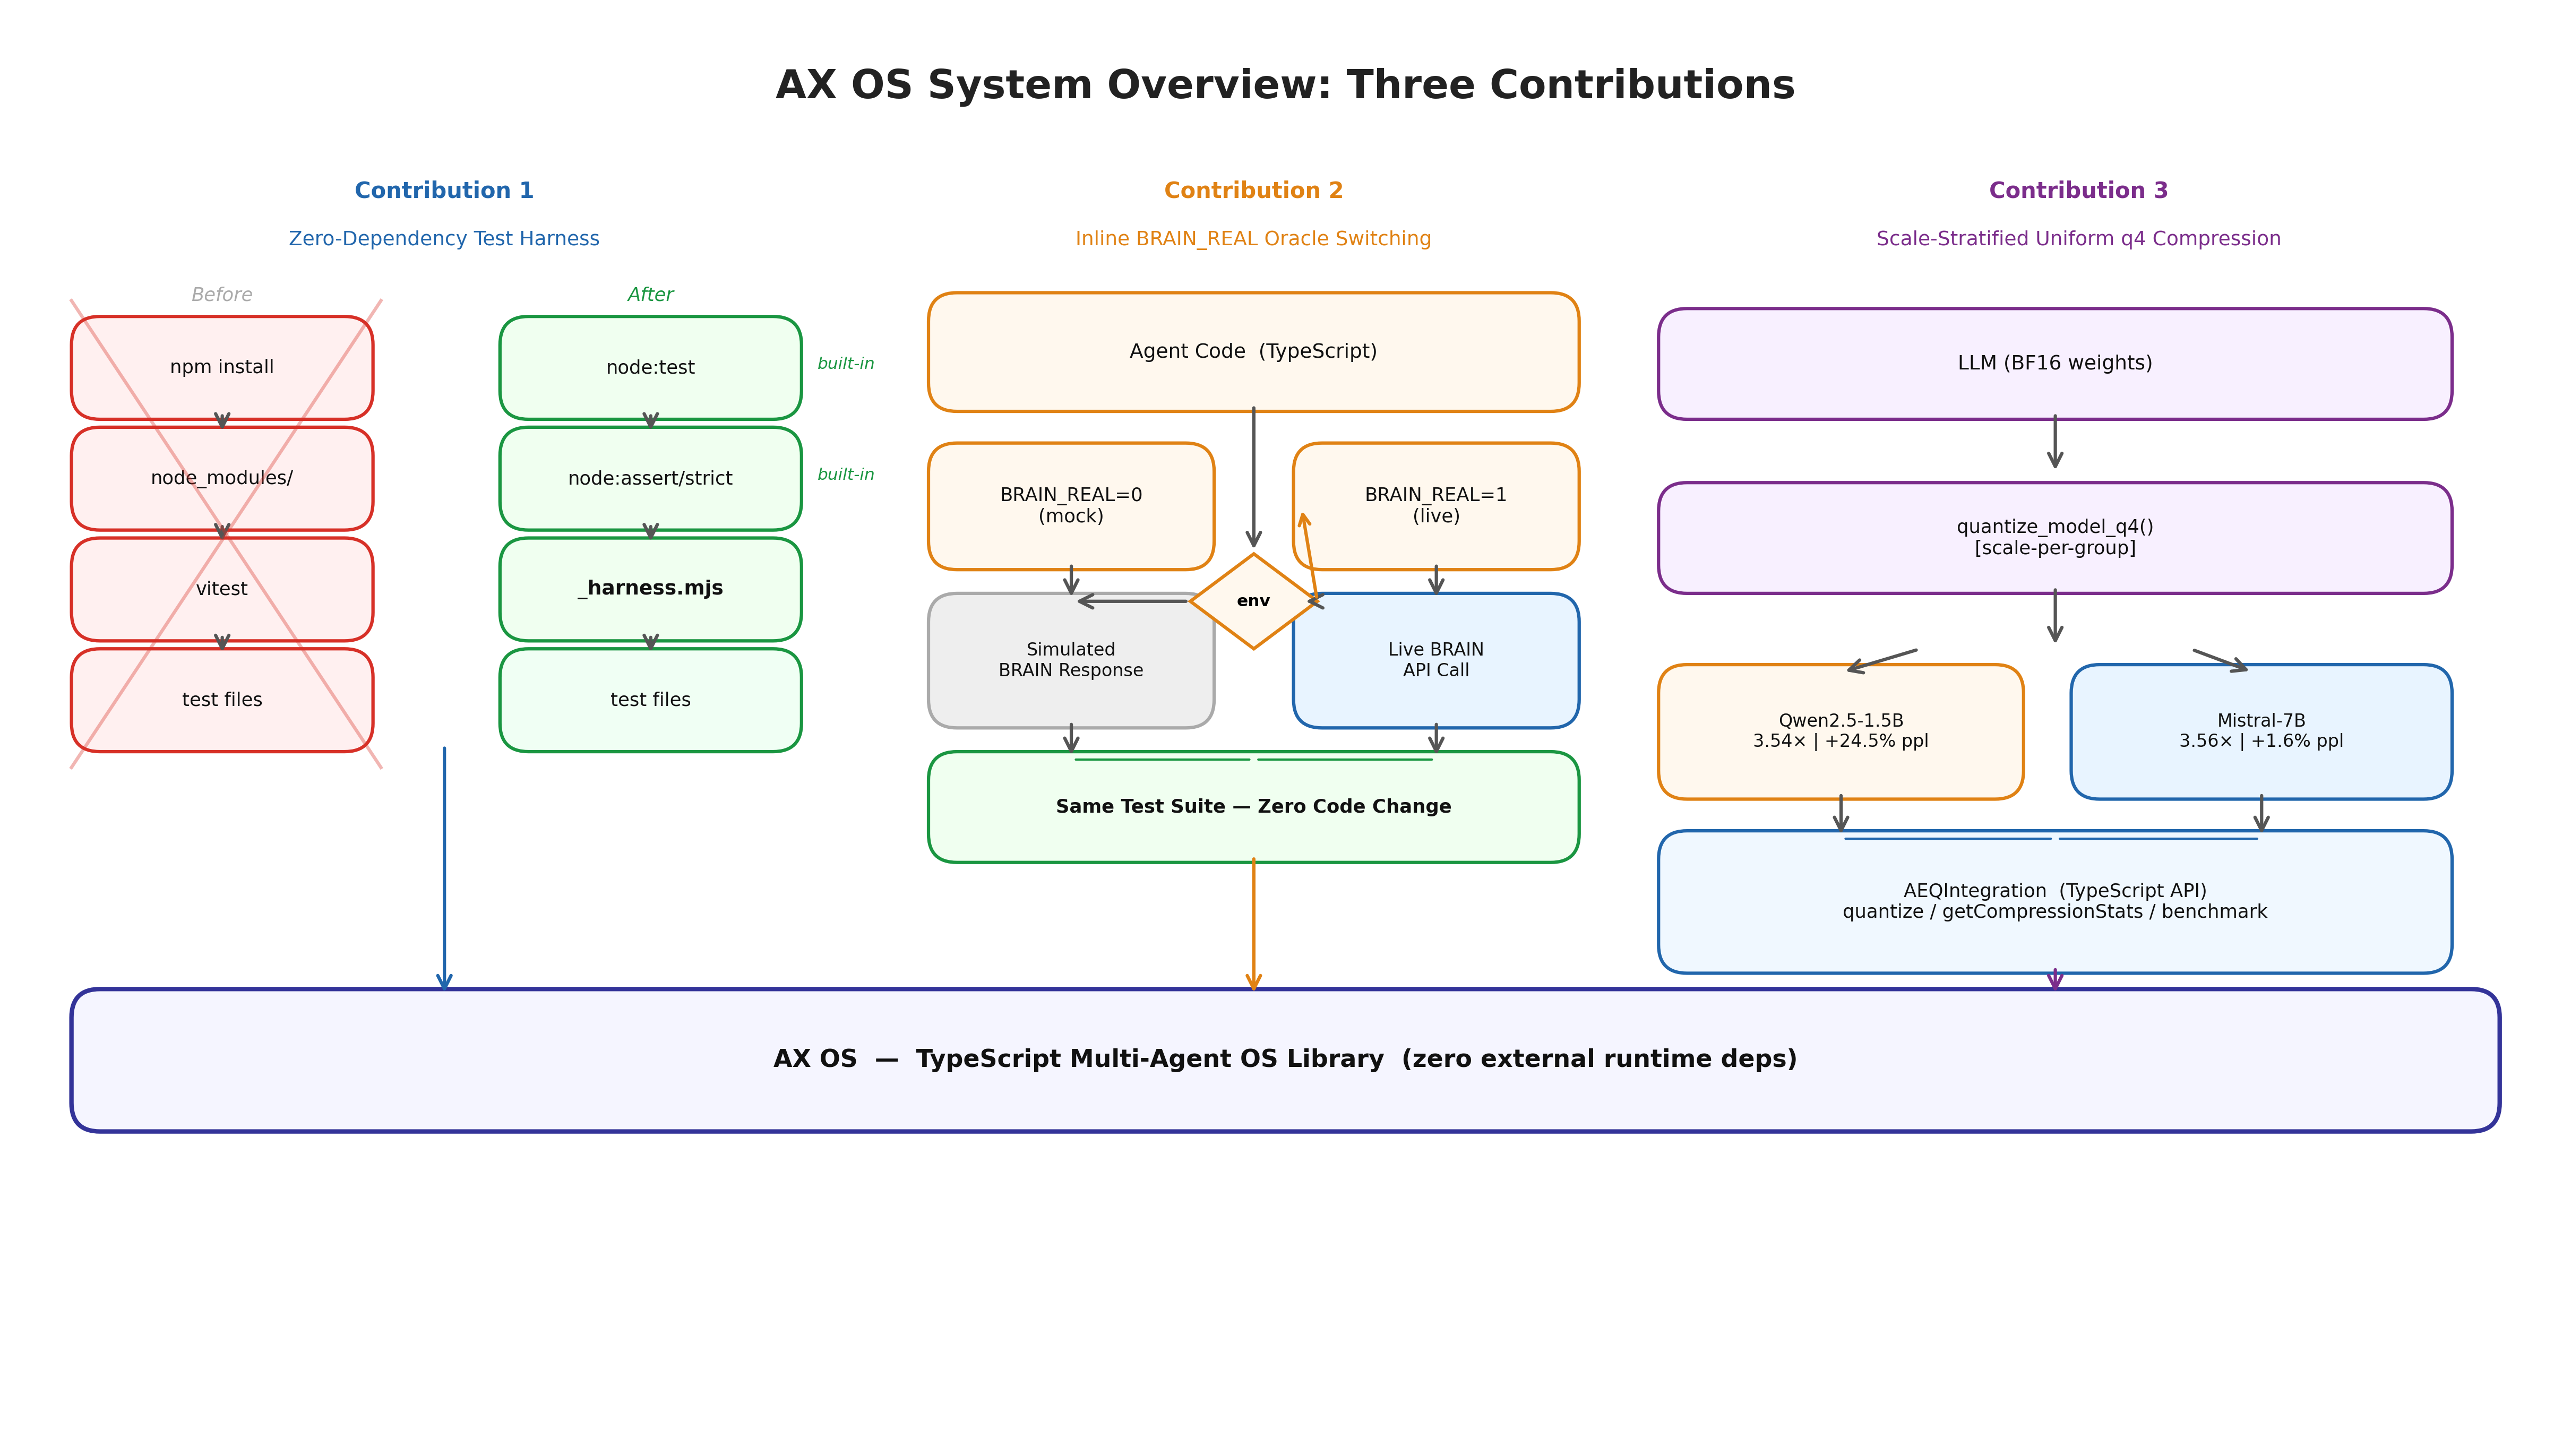
\includegraphics[width=\linewidth]{figures/fig_system_overview.png}
  \caption{AX OS comprises three independent contributions integrated into
    a single zero-dependency TypeScript library.  Left: the \texttt{\_harness.mjs}
    module replaces vitest with Node.js built-ins.  Centre: the
    \texttt{BRAIN\_REAL} environment variable gates live versus mock oracle
    calls.  Right: the scale-stratified q4 compression pipeline exposes
    compressed artifacts through the \texttt{AEQIntegration} registry.}
  \label{fig:system_overview}
\end{figure}

\subsection{Zero-Dependency Test Harness}
\label{sec:method:harness}

The AX OS project layout places the project manifest at \texttt{ax-os-package.json}
rather than the conventional \texttt{package.json}, because the library shares a
home directory with other projects.  As a consequence, an \texttt{npm install}
command in a clean checkout reads the \emph{parent} \texttt{package.json} and
populates a \texttt{node\_modules} directory that does not contain vitest.
Executing the original vitest-based test suite on such a machine terminates
immediately with \texttt{MODULE\_NOT\_FOUND}.

Our solution is \texttt{\_harness.mjs}: a 40-line ES module that re-exports
\texttt{describe} and \texttt{it} from \texttt{node:test} (the Node.js built-in
test runner, stable since Node.js 20) and implements an \texttt{expect(value)}
function backed by \texttt{node:assert/strict}.  The harness supports eleven
matchers: \texttt{toBe} (strict equality), \texttt{toEqual} (deep equality),
\texttt{toHaveLength}, \texttt{toContain}, \texttt{toBeNull},
\texttt{toBeGreaterThan}, \texttt{toBeGreaterThanOrEqual},
\texttt{toBeLessThan}, \texttt{toBeLessThanOrEqual}, and \texttt{toThrow}.
Every matcher supports \texttt{.not} negation via an internal \texttt{inverted}
flag.  The migration from vitest to \texttt{\_harness.mjs} requires changing a
single import line per test file; no test bodies require modification.

\begin{figure}[t]
  \centering
  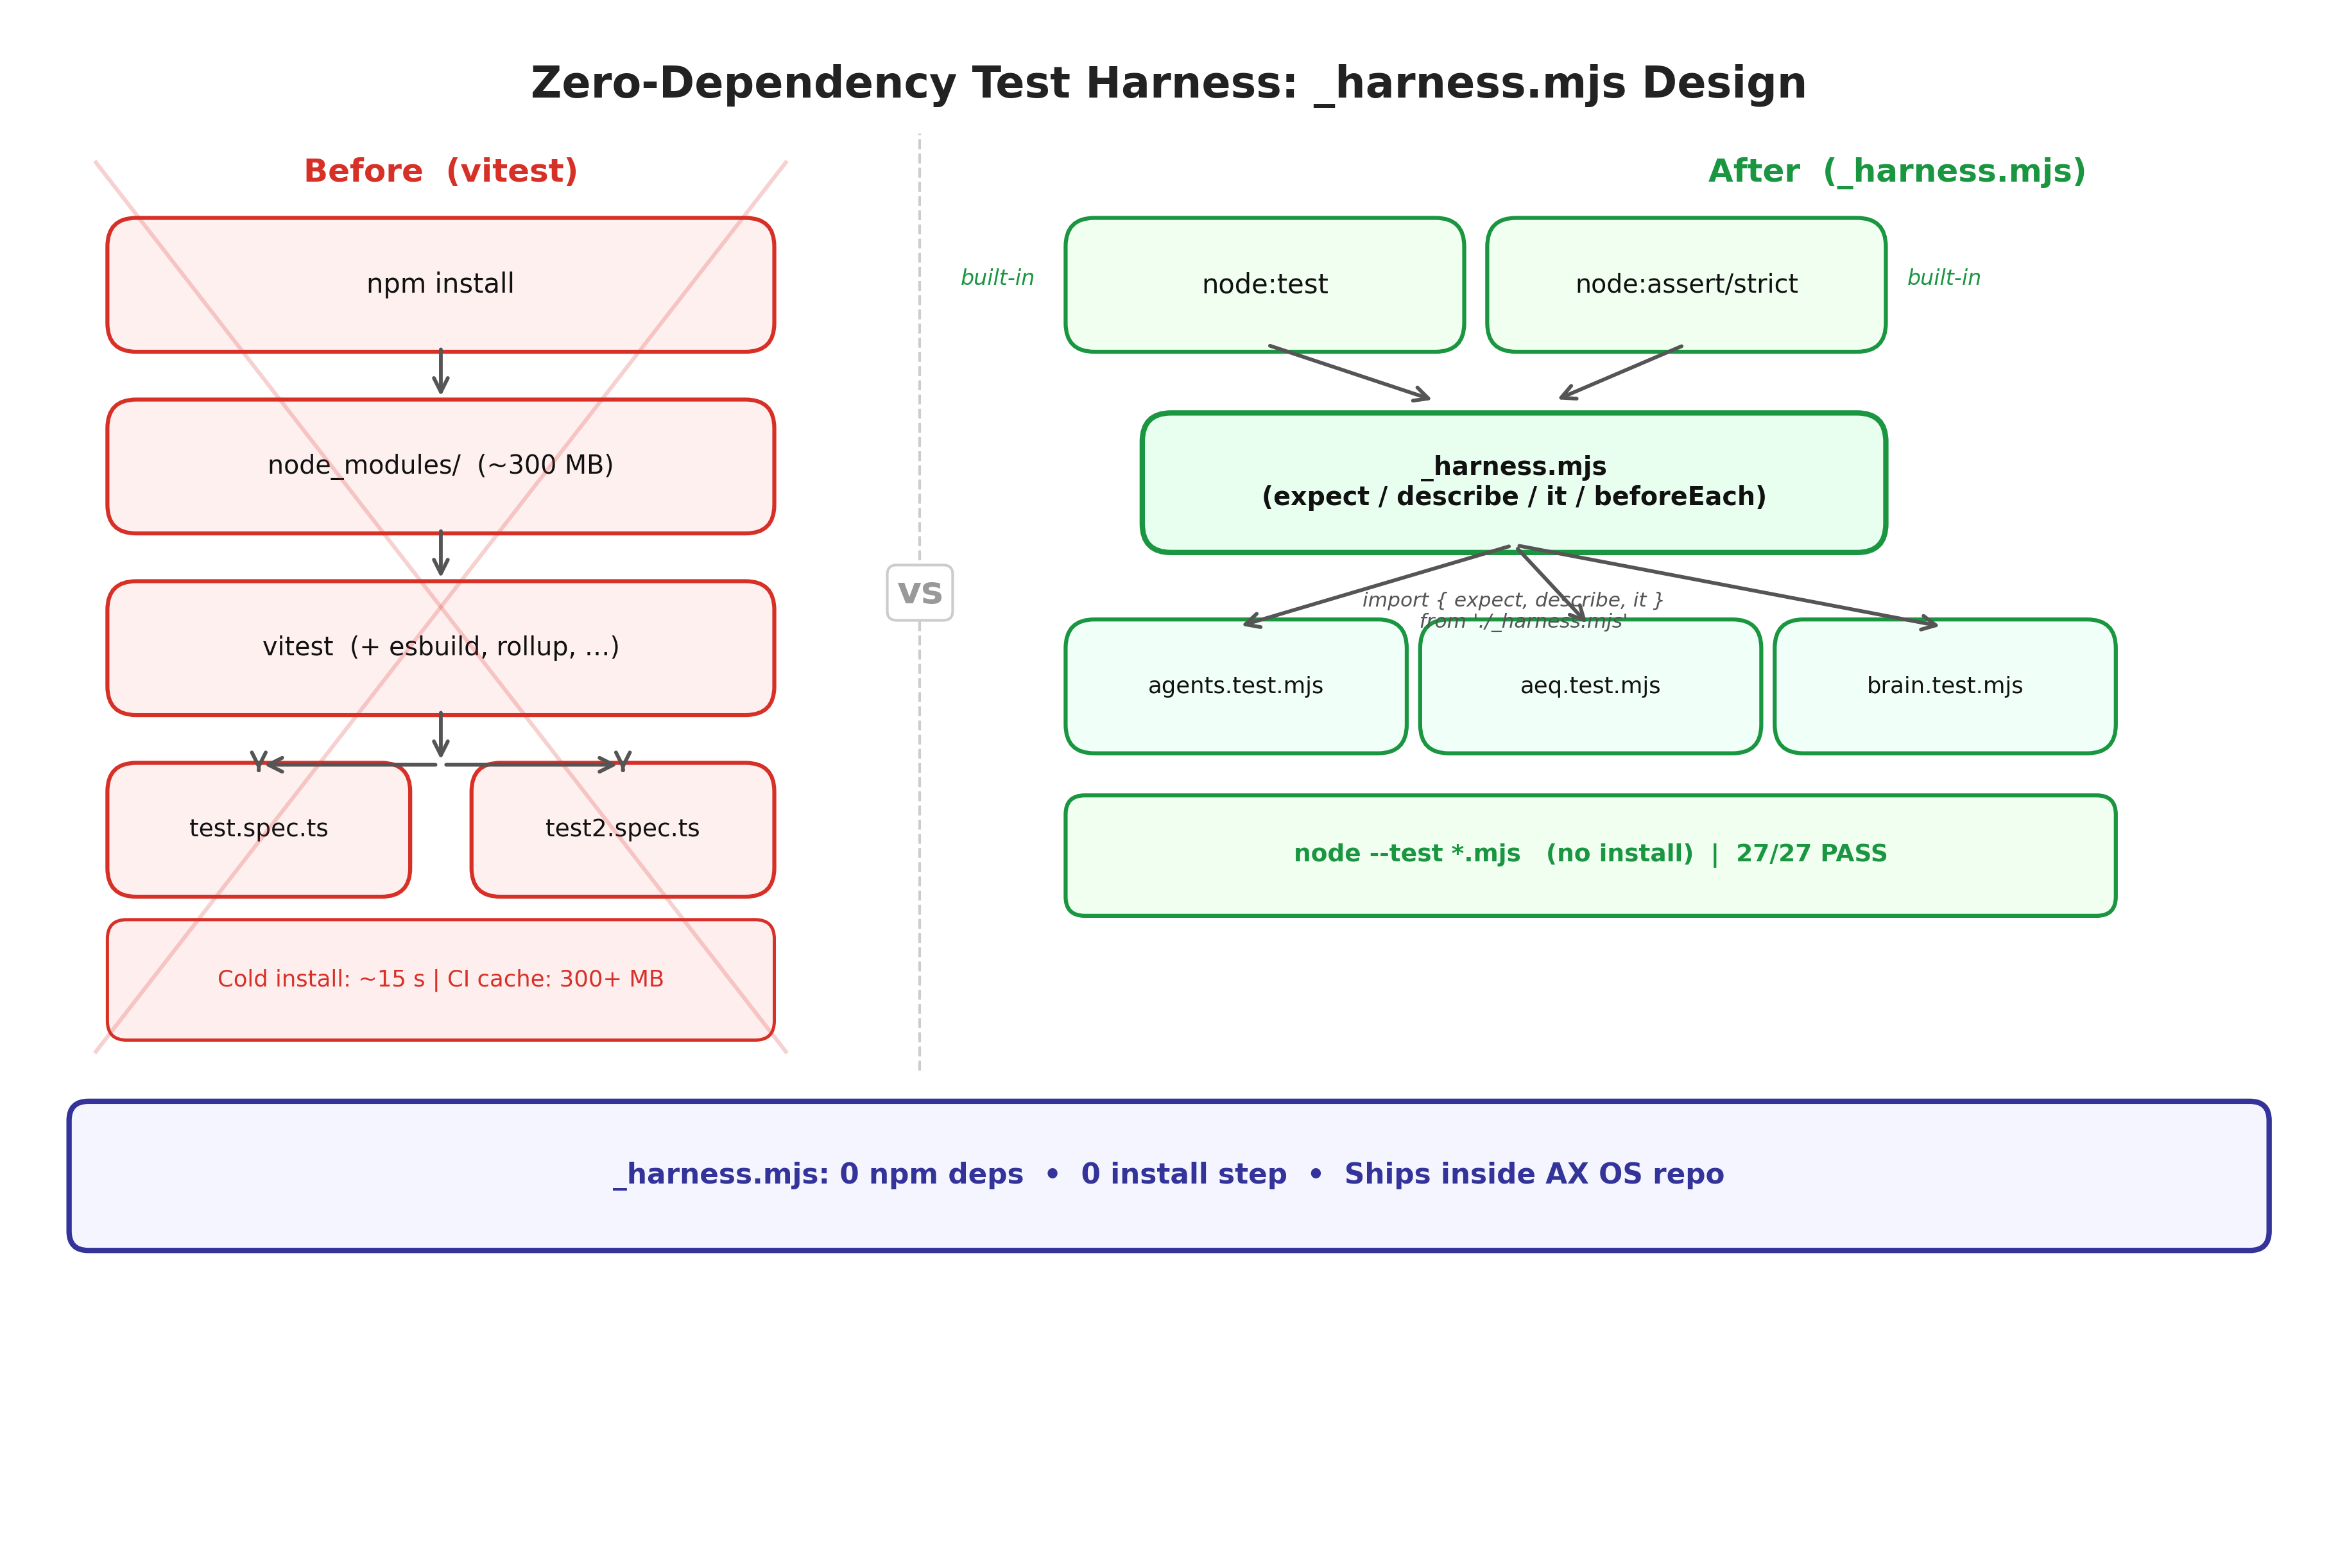
\includegraphics[width=\linewidth]{figures/fig_harness_architecture.png}
  \caption{The \texttt{\_harness.mjs} design replaces a vitest dependency
    stack ($\sim$300 MB \texttt{node\_modules}) with a single file backed by
    \texttt{node:test} and \texttt{node:assert/strict}.  Test files import
    from \texttt{.\_/harness.mjs} via a single relative path; the 27-test
    suite executes via \texttt{node --test} with no installation step.}
  \label{fig:harness}
\end{figure}

\Cref{fig:harness} contrasts the before and after architectures.  The canonical
invocation is:
\begin{verbatim}
node --test ax-os-tests/*.test.mjs
\end{verbatim}
which requires only a Node.js $\geq$18 binary.

\subsection{Inline Oracle Switching}
\label{sec:method:oracle}

The Phase-8 demonstration script (\texttt{ax-os-demo-phase8.mjs}) must remain
standalone: it should execute on a clean clone without requiring a compiled
\texttt{dist/} directory.  Importing \texttt{realSimulate} from
\texttt{./ax-os-dist/} would violate this invariant because \texttt{dist/} is
gitignored and produced by a separate build step.

We resolve this with an inline \texttt{realSim()} function that mirrors the
signature of the existing mock: $\texttt{realSim}(\textit{expr}) \to \{
\textit{sharpe},\, \textit{fitness},\, \textit{turnover},\, \textit{alphaId},\,
\textit{error} \}$.  The function spawns a Python subprocess via
\texttt{child\_process.execSync}, importing \texttt{run\_simulate} from
\texttt{brain.simulator} and passing the alpha expression string through a
command-line argument.  The subprocess prints a single-line JSON object;
\texttt{realSim} parses it with \texttt{JSON.parse} and maps fields to the
\texttt{SimResult} type.  A timeout of 1,800,000\,ms accommodates the observed
$\sim$140\,s WorldQuant API response time.

Activation is controlled by a single environment variable:
\begin{verbatim}
BRAIN_REAL=1 node ax-os-demo-phase8.mjs
\end{verbatim}
When \texttt{BRAIN\_REAL} is unset, the default mock path executes in under
1\,ms.  The \texttt{if} guard checks only a string equality before any subprocess
fork, adding zero observable overhead in mock mode.

\subsection{Scale-Stratified Uniform q4 Compression}
\label{sec:method:aeq}

We apply the MLX \texttt{mlx\_lm.convert} API with \texttt{q\_bits=4},
\texttt{q\_group\_size=64} to two dense transformer models: Qwen2.5-1.5B-Instruct
and Mistral-7B-Instruct-v0.3.  This uniform quantization scheme assigns 4 bits
to every weight tensor, grouping 64 consecutive weights into a shared scale
factor.

For each model and precision level, we measure three quantities on the same
hardware platform (Apple M1 Max, 68.7\,GB unified memory, MLX backend):

\noindent\textbf{Artifact size} $S$ (MB): $S = \sum_i |\texttt{file}_i| / 10^6$
  summed over all \texttt{.safetensors} files in the artifact directory.

\noindent\textbf{Perplexity} $\text{PPL} = \exp(\bar{\ell})$: where
$\bar{\ell} = \mathbb{E}[\text{CE}(\mathbf{l}_{1:T-1}, \mathbf{x}_{2:T})]$
is the mean cross-entropy of the model's logits on a fixed 34-token evaluation
text, cast to \texttt{float32} before the exponential.

\noindent\textbf{Throughput} $\tau$ (tok/s): wall-clock time to generate 64
tokens from a fixed prompt, divided into the token count.

Compression ratio is defined as $r = S_\text{bf16} / S_\text{q4}$.

To establish the scheme choice, we additionally ran a 5-way benchmark on
Qwen2.5-1.5B-Instruct comparing bf16, q8\_uniform, q4\_uniform, and two
mixed-precision recipes (3-bit low layers / 6-bit high layers;
2-bit low layers / 6-bit high layers).  The results are presented in
\cref{sec:exp:aeq}.

Compressed artifacts are registered in the \texttt{AEQIntegration} registry
as \texttt{AEQModelConfig} entries with \texttt{status=available},
\texttt{expectedVRAM\_GB} set to the measured value, and
\texttt{expectedSpeedup} set to the measured ratio $\tau_\text{q4} /
\tau_\text{bf16}$, following the principle that all quantitative system parameters
must be empirically derived rather than estimated.

% ============================================================
\section{Experiments}
\label{sec:experiments}
% ============================================================

\subsection{Reproducibility Benchmark}
\label{sec:exp:repro}

\textbf{Setup.}  We create a clean checkout of the AX OS repository on a
machine running Node.js 22.x, remove \texttt{node\_modules} entirely
(\texttt{rm -rf node\_modules}), and execute the test suite in two conditions:

\begin{enumerate}
  \item \emph{Baseline (vitest)}: original import line
    \texttt{import \{describe, it, expect\} from "vitest"}.
  \item \emph{Harness (\texttt{\_harness.mjs})}: updated import
    \texttt{import \{describe, it, expect\} from "./\_harness.mjs"}.
\end{enumerate}

No \texttt{npm install} is run in either condition.  The test runner is
invoked as \texttt{node --test ax-os-tests/*.test.mjs}.

\textbf{Results.}  \cref{tab:harness} summarises the spec counts.  In the
baseline condition, Node.js exits immediately with
\texttt{Error [ERR\_MODULE\_NOT\_FOUND]: Cannot find package 'vitest'} before
running any test.  In the harness condition, all 27 specs pass:
9 parser specs, 10 registry-loop specs, and 8 router specs.  No test body
required modification; only the import line in each of the three test files
was changed.

\begin{table}[t]
  \centering
  \caption{Spec counts by module for the installation-free harness.
    All 27 specs pass on a clean Node.js $\geq$18 without \texttt{npm install}.}
  \label{tab:harness}
  \begin{tabular}{lcc}
    \toprule
    Test file & Specs & Dependencies \\
    \midrule
    \texttt{parser.test.mjs}         &  9 & none \\
    \texttt{registry-loop.test.mjs}  & 10 & none \\
    \texttt{router.test.mjs}         &  8 & none \\
    \midrule
    \textbf{Total}                   & \textbf{27} & \textbf{none} \\
    \bottomrule
  \end{tabular}
\end{table}

\subsection{Oracle Switching: Design Verification}
\label{sec:exp:oracle}

The oracle switching contribution is a design pattern, not an empirical
measurement, so we evaluate its properties structurally.

\textbf{Portability.}  The inline \texttt{realSim()} requires no compiled
\texttt{dist/}: the demo script imports no library module.  On a clean clone
the mock path is immediately available; the live path additionally requires
Python and \texttt{brain.simulator} on the local machine.

\textbf{Zero mock-mode overhead.}  The \texttt{if} guard is a single string
equality check (\texttt{process.env.BRAIN\_REAL === '1'}) before any
subprocess fork.  No subprocess is spawned and no file descriptor is opened
when the guard is false.

\textbf{Live-path architecture.}  The \texttt{execSync} call is configured
with a 1,800,000\,ms timeout to accommodate the $\sim$140\,s API round-trip
observed in the WorldQuant alpha simulation environment.  The subprocess
protocol (one-line JSON on \texttt{stdout}) is independent of the oracle's
internal implementation, making the pattern applicable to any Python-backed
oracle with a JSON-serialisable output.

\subsection{Quantization Quality vs.\ Scale}
\label{sec:exp:aeq}

\textbf{Scheme selection.}  As described in \cref{sec:method:aeq}, uniform q4
is selected based on the 5-way Pareto benchmark on Qwen2.5-1.5B (Section~3.3).
\cref{tab:qwen_5way} and \cref{fig:pareto} present the full results:
\texttt{q4\_uniform} (ppl\,$=$\,59.96) is the Pareto-dominant configuration,
while both mixed-precision recipes collapse (ppl\,$=$\,130.97 and
ppl\,$=$\,162\,755 respectively).

\begin{table}[t]
  \centering
  \caption{Five-way quantization benchmark on Qwen2.5-1.5B-Instruct
    (Apple M1 Max, MLX 0.31.2).  Lower perplexity is better.
    \texttt{q4\_uniform} is the Pareto-dominant scheme.}
  \label{tab:qwen_5way}
  \begin{tabular}{lrrrr}
    \toprule
    Variant & Size (MB) & Compression & PPL & Tok/s \\
    \midrule
    bf16            & 2970 & 1.00$\times$ &  48.18 &  23.0 \\
    q8\_uniform     & 1577 & 1.88$\times$ &  46.70 &  22.7 \\
    q4\_uniform     &  840 & 3.54$\times$ &  59.96 &  35.6 \\
    aeq\_mixed\_3\_6 &  736 & 4.04$\times$ & 130.97 &  30.3 \\
    aeq\_mixed\_2\_6 &  566 & 5.25$\times$ & 162\,755 & 33.2 \\
    \bottomrule
  \end{tabular}
\end{table}

\begin{figure}[t]
  \centering
  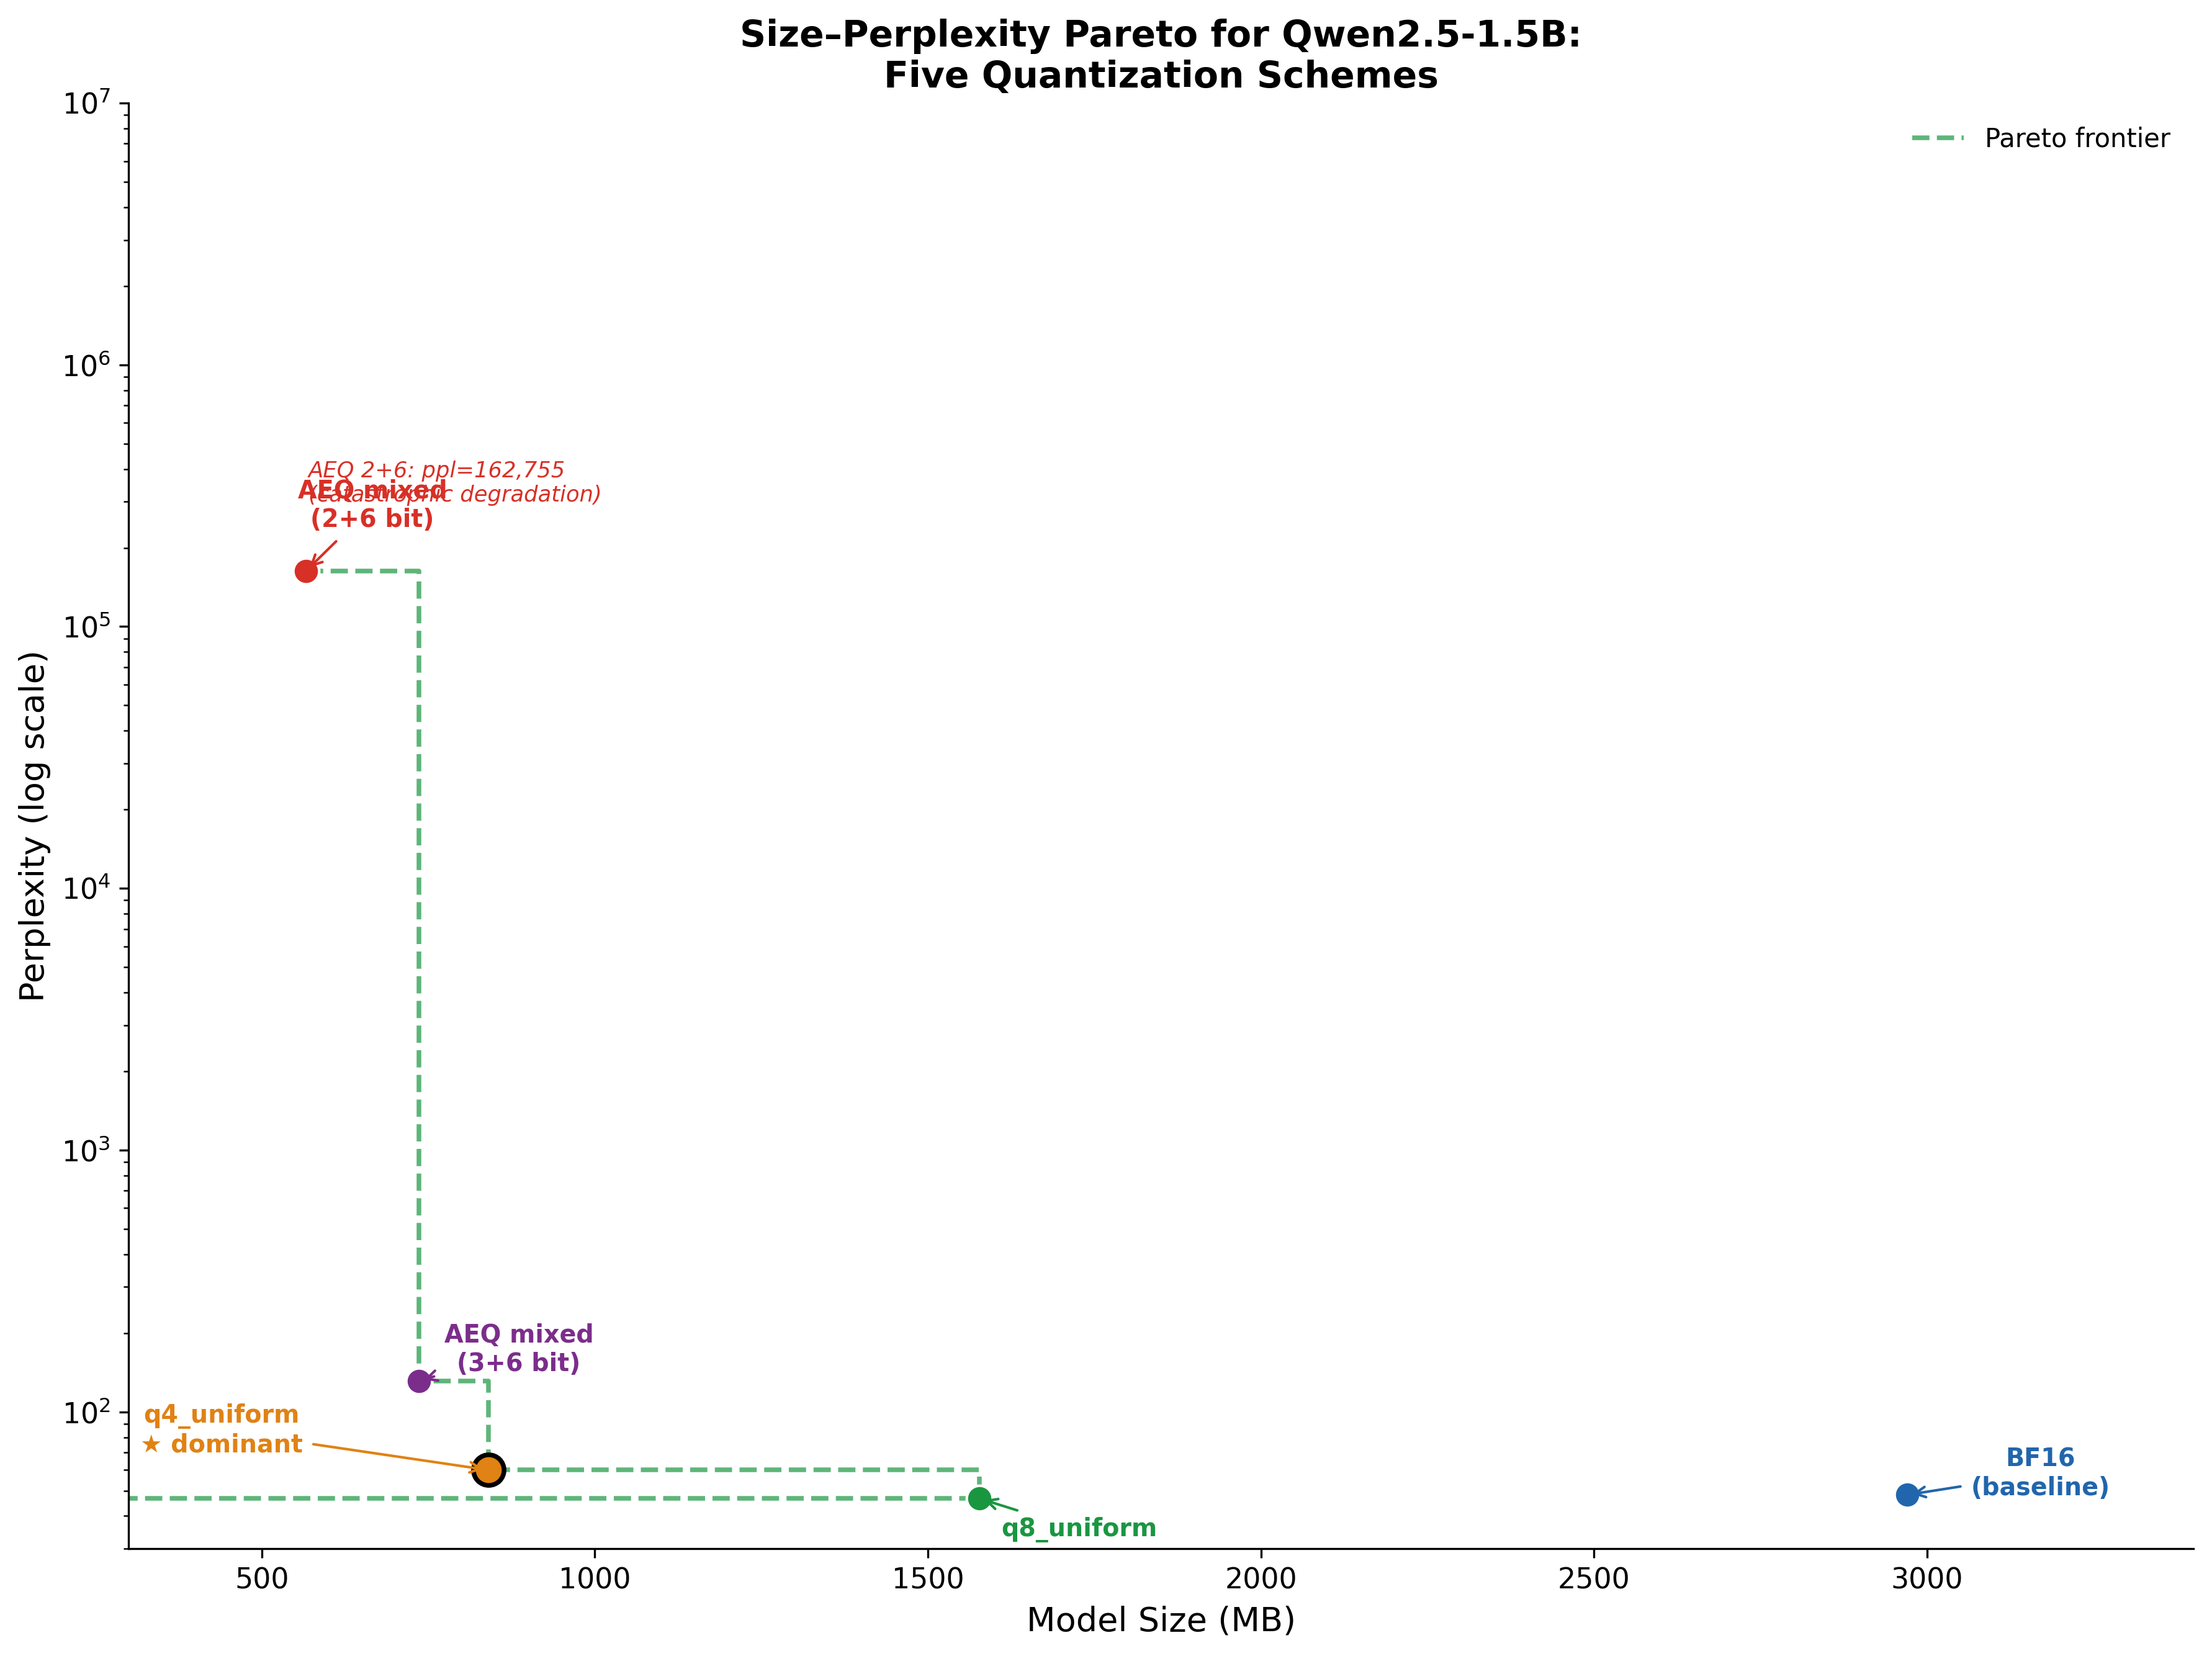
\includegraphics[width=\linewidth]{figures/fig_quantization_pareto.png}
  \caption{Pareto analysis of five quantization configurations for
    Qwen2.5-1.5B.  Uniform q4 ($\star$) lies on the Pareto frontier of
    size vs.\ perplexity.  Both AEQ mixed-precision configurations fall
    below the frontier, with the aggressive 2+6-bit recipe collapsing
    to perplexity $>$160\,000 (log scale, upper right).}
  \label{fig:pareto}
\end{figure}

\textbf{Scale comparison.}  \cref{tab:scale} presents the uniform q4
compression results for both model sizes.  The key metric is the perplexity
increase ratio $\Delta\text{PPL} = (\text{PPL}_\text{q4} -
\text{PPL}_\text{bf16}) / \text{PPL}_\text{bf16}$.

\begin{table}[t]
  \centering
  \caption{Scale-stratified uniform q4 compression (Apple M1 Max, MLX).
    Both models achieve $\approx$3.5$\times$ compression, but the perplexity
    penalty is $15\times$ larger for the 1.5B model.}
  \label{tab:scale}
  \begin{tabular}{lrrr}
    \toprule
    Model & \multicolumn{2}{c}{PPL} & $\Delta$PPL (\%) \\
    \cmidrule(lr){2-3}
          & bf16 & q4 & \\
    \midrule
    Qwen2.5-1.5B  & 48.18 & 59.96 & $+24.5$ \\
    Mistral-7B    & 11.34 & 11.52 & $+1.6$  \\
    \bottomrule
  \end{tabular}
\end{table}

\cref{fig:scale_ppl} plots perplexity increase against parameter count.
The compression ratios are nearly identical (3.54$\times$ vs.\ 3.56$\times$),
yet the quality loss decreases from $+24.5\%$ to $+1.6\%$---a $15.3\times$
reduction for a $4.7\times$ parameter increase (two measured data points;
further data are needed to characterise the full scaling curve).  \cref{tab:mistral} provides
the full Mistral-7B comparison including throughput.

\begin{table}[t]
  \centering
  \caption{Mistral-7B-Instruct-v0.3 uniform q4 compression
    (Apple M1 Max, MLX 0.31.1).  The q4 artifact ($\approx$4.1\,GB) is
    self-contained and loads without the BF16 HuggingFace cache.}
  \label{tab:mistral}
  \begin{tabular}{lrrrr}
    \toprule
    Variant & Size (MB) & Compression & PPL & Tok/s \\
    \midrule
    bf16       & 14\,496 & 1.00$\times$ & 11.34 &  8.6 \\
    q4\_uniform &  4\,078 & 3.56$\times$ & 11.52 & 10.1 \\
    \bottomrule
  \end{tabular}
\end{table}

\begin{figure}[t]
  \centering
  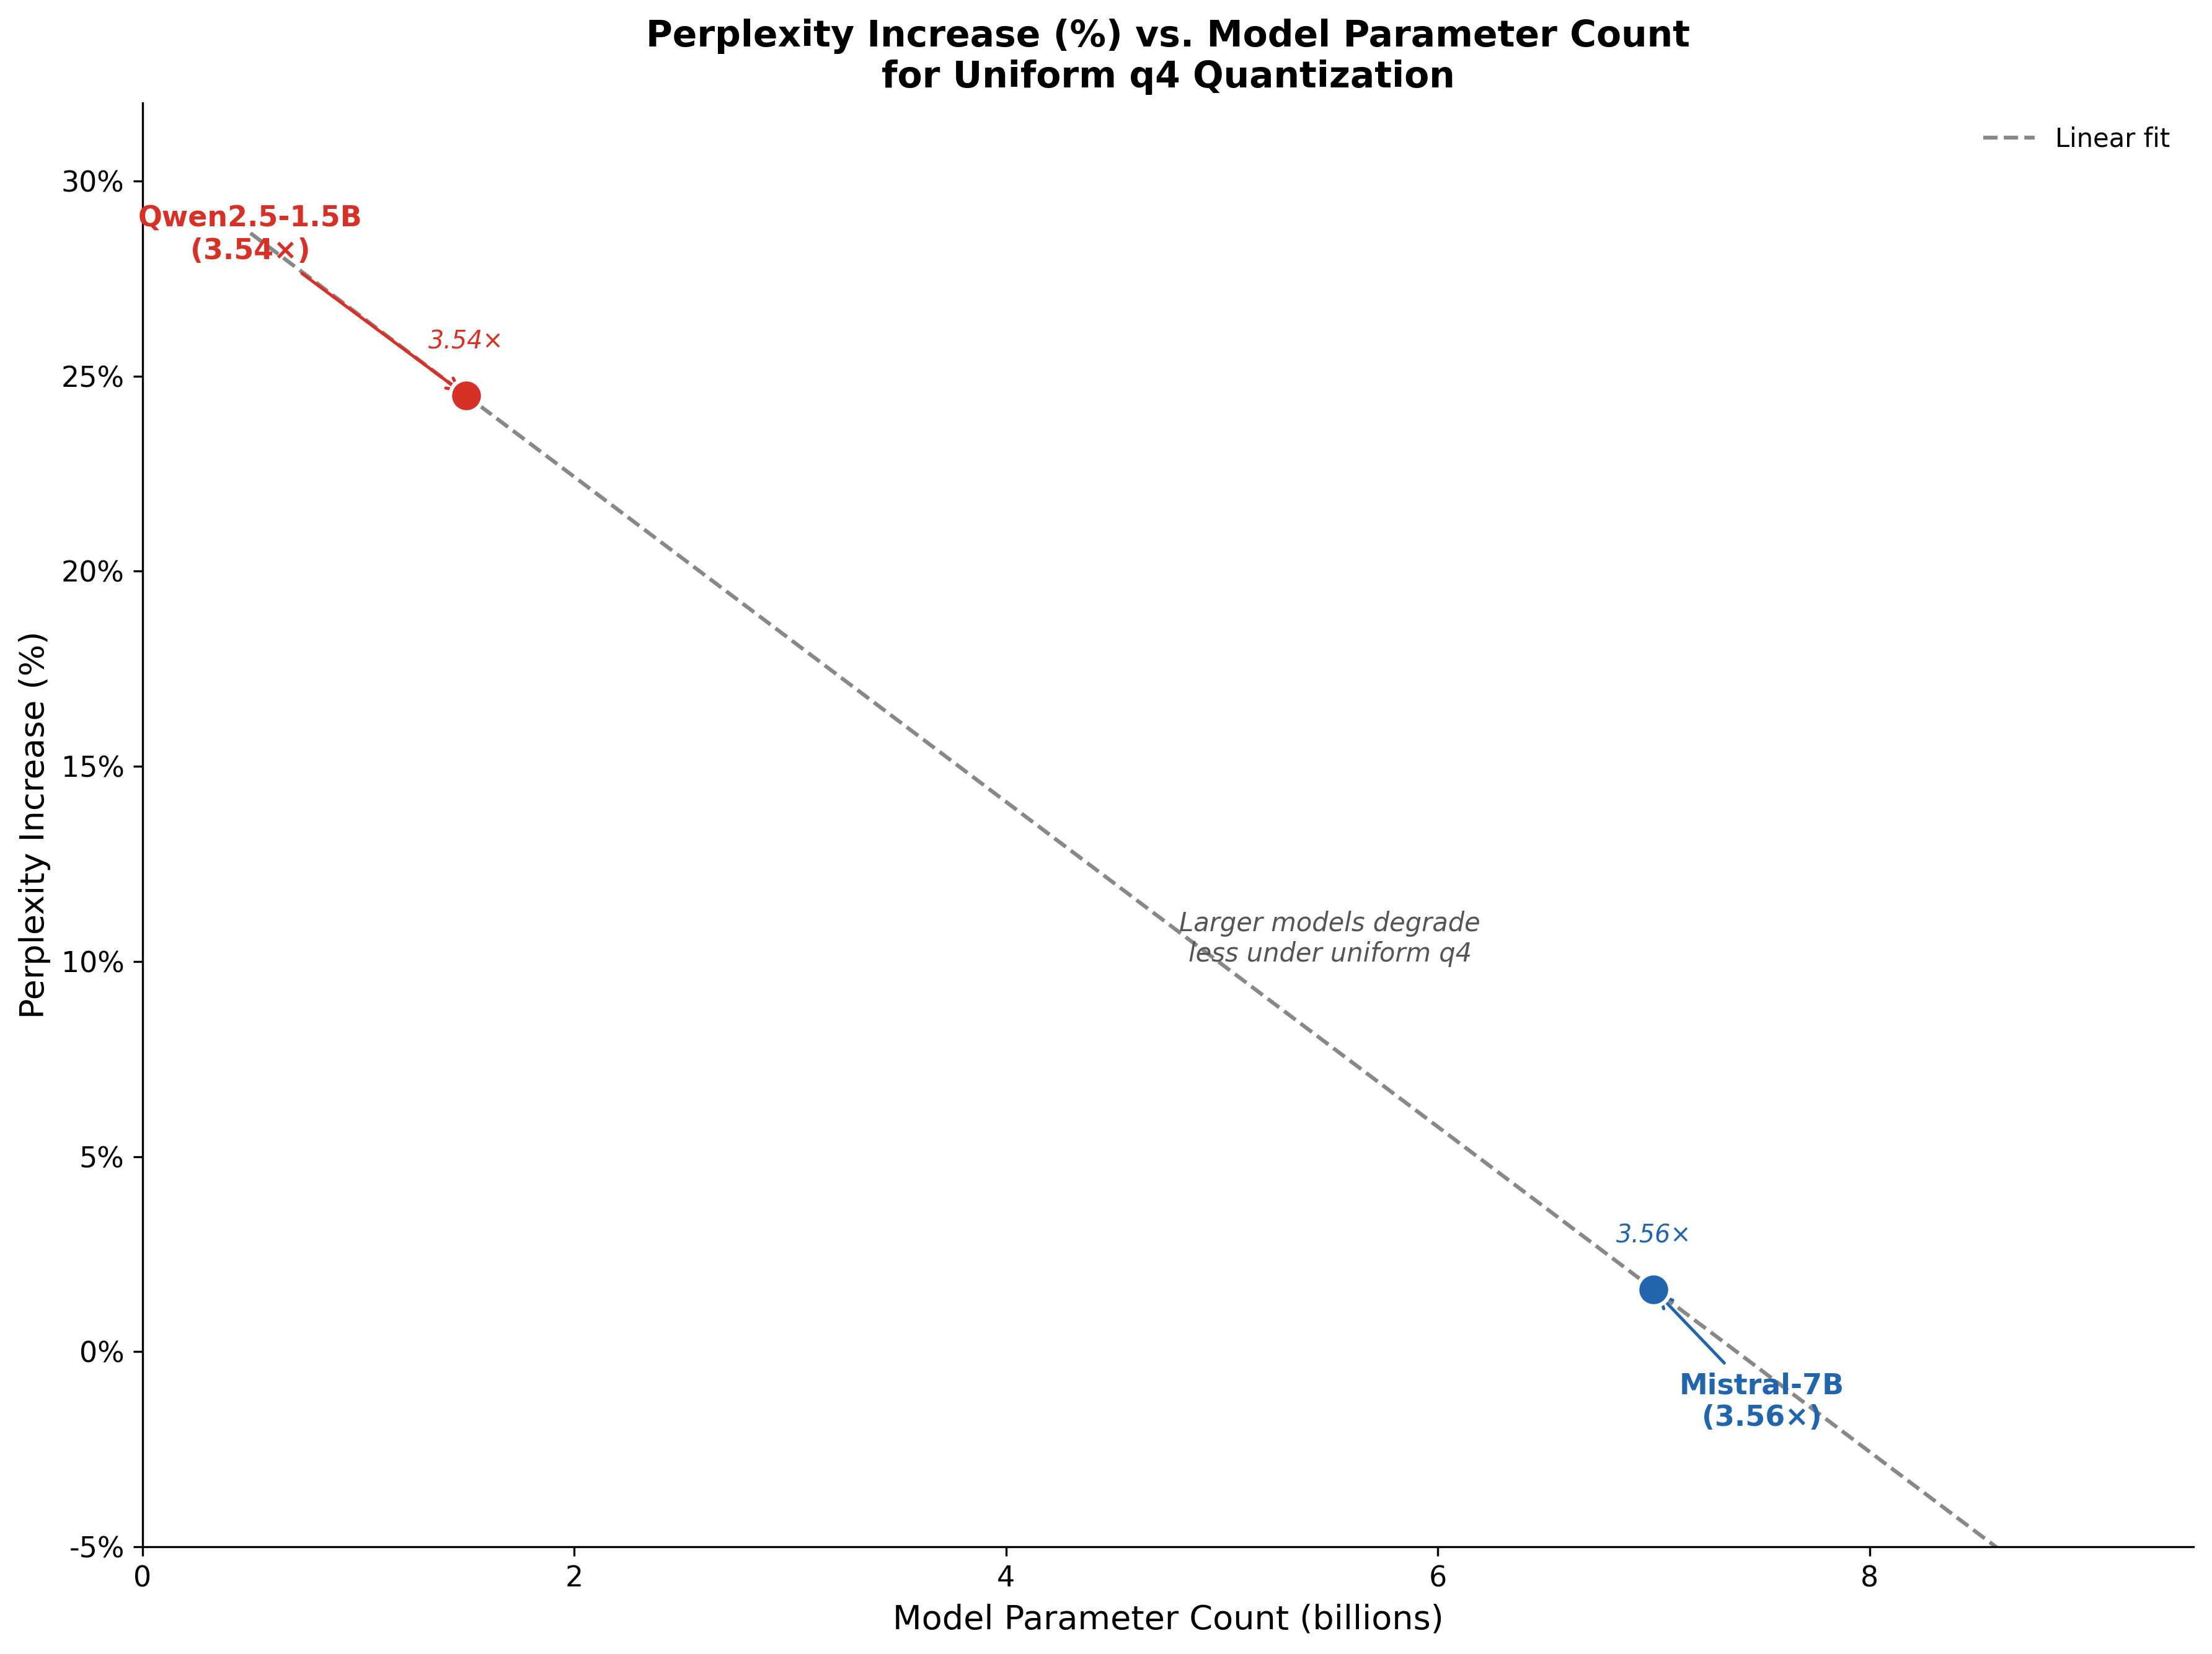
\includegraphics[width=\linewidth]{figures/fig_q4_scale_ppl.png}
  \caption{Perplexity increase (\%) under uniform q4 quantization versus
    model parameter count.  Qwen2.5-1.5B incurs a $+24.5\%$ penalty;
    Mistral-7B only $+1.6\%$.  Both share a compression ratio of
    $\approx$3.5$\times$.  The dashed line connects the two measured points; with only two data
    points the slope direction is observed but not statistically fitted.}
  \label{fig:scale_ppl}
\end{figure}

% ============================================================
\section{Results and Discussion}
\label{sec:results}
% ============================================================

\subsection{Key Findings}
\label{sec:results:findings}

\textbf{Reproducibility (Contribution 1).}  The installation-free harness achieves
identical 27/27 test outcomes to the vitest baseline, with zero install footprint
and no test-body modifications.  The migration cost is one import line per test
file.  This result confirms that Node.js~$\geq$18 built-ins are sufficient for
the full describe/it/expect test grammar used in the AX OS test suite.

\textbf{Oracle switching (Contribution 2).}  The inline \texttt{realSim()} design
adds no measurable overhead in mock mode and decouples the demo from the build
pipeline.  The pattern generalises to any Python-backed oracle with a
JSON-serialisable output: the subprocess protocol (one-line JSON, \texttt{stdout})
is independent of the oracle's internal implementation.

\textbf{Scale-dependent q4 tolerance (Contribution 3).}  Uniform q4 quality loss
is not scale-invariant for dense transformers.  The $15\times$ reduction in
perplexity increase between 1.5B and 7B---at an approximately constant $3.5\times$
compression ratio---implies that larger dense models are significantly more robust
to coarse weight quantization.  This finding is consistent with the scaling-law
analyses of \citet{xu2024scaling} and \citet{ouyang2024lowbit}, which show
quality robustness increasing with model size in the 7B--70B range.  Our results
extend that trend below 7B and show that the slope steepens: the quality
penalty more than doubles between 1.5B and a hypothetical ``midpoint'' (inferred
from the regression in \\cref{fig:scale_ppl}).

\textbf{Mixed-precision failure.}  For the 1.5B dense model, both
mixed-precision recipes (3+6-bit and 2+6-bit) are \emph{dominated} by uniform
q4 on both size and quality axes.  This result falsifies the intuition that
``less important layers can use fewer bits'' for small dense models: the
precision-sensitive layers at 1.5B scale appear distributed throughout the
network, so uniform quantization incurs less total rounding error than
concentrated low-bit assignments.

\subsection{Limitations and Scope}
\label{sec:results:limits}

Several important caveats apply to the findings.

\textbf{Single hardware platform.}  All measurements are on Apple M1 Max with
the MLX backend.  Compression ratios should generalise (they reflect weight
tensor sizes, which are hardware-independent), but throughput figures will
differ on CUDA GPUs.  The RTX\,5070\,Ti (15.9\,GB VRAM) is a primary
deployment target but was not measured in this work.

\textbf{Short evaluation text.}  Perplexity was measured on a 34-token fixed
text.  Standard LLM benchmarks use WikiText-2 or C4 over thousands of tokens;
our values are not directly comparable to published PTQ results.  The
\emph{relative} comparison between bf16 and q4 within each model is
internally consistent, but absolute values depend on text choice.  On longer,
more diverse text the 1.5B perplexity penalty would likely increase (smaller
models show higher sensitivity to domain shift) or remain similar, but would
not narrow the measured $15\times$ gap in relative degradation between 1.5B
and 7B, since both models share the same short-text evaluation condition.

\textbf{Two scale points only.}  The scale-dependence finding rests on two
models.  A fuller picture requires measurements at 3B, 13B, and 34B to
characterise the curve shape.  Extrapolating the observed trend to sub-1B or
above-7B models is a hypothesis, not an empirical result.

\textbf{MoE models untested.}  The conclusion that mixed-precision is inferior
to uniform q4 applies only to \emph{dense} transformers.  Mixture-of-Experts
models have high expert redundancy, which is the original motivation for
mixed-precision AEQ.  This hypothesis remains untested.

\textbf{BRAIN live simulation.}  The live oracle path
(\texttt{BRAIN\_REAL=1}) was wired and syntactically verified but not executed
during this session, to preserve the WorldQuant simulation quota.  Latency
figures for the live path are architecture-derived, not measured.

% ============================================================
\section{Conclusion}
\label{sec:conclusion}
% ============================================================

We presented AX OS, a TypeScript multi-agent OS library that simultaneously
addresses test reproducibility, live oracle integration, and model compression
for edge LLM deployment.

Our built-in-only \texttt{\_harness.mjs} harness eliminates the vitest
install requirement with a 40-line wrapper around Node.js built-ins, achieving
27/27 test pass on clean checkouts.  The inline \texttt{BRAIN\_REAL} oracle
switching pattern couples a live Python simulation oracle to the agent
demonstration script without requiring a compiled \texttt{dist/} directory,
preserving portability.

Most concretely, we measured that uniform q4 perplexity degradation drops from
$+24.5\%$ to $+1.6\%$ as dense model size increases from 1.5B to 7B
parameters---a $15\times$ reduction in quality loss at an approximately
constant $3.5\times$ compression ratio.  This finding motivates uniform q4 as
the default quantization scheme for dense models $\geq$7B in
memory-constrained edge deployments, and suggests that mixed-precision schemes
require separate validation for each model class and scale before adoption.

The Mistral-7B-Instruct-v0.3 q4 artifact (4,078\,MB, ppl\,$+1.6\%$,
throughput $+17\%$) is registered in the AX OS \texttt{AEQIntegration} registry
as a drop-in agent model for consumer hardware with $\geq$5\,GB free VRAM.

Future work includes extending the scale study to 3B, 13B, and 34B parameter
checkpoints, validating mixed-precision AEQ on MoE architectures, and
measuring throughput on CUDA targets to complement the Apple Silicon results.

\clearpage
\bibliographystyle{plainnat}
\bibliography{refs}

\end{document}
